\chapter{Approach}

\section{Architecture}

The backend is considered as the software and database that runs on a dedicated server. The Frontend/Client communicates with the Backend via an Interface described below.

\section{Technologies}

In the following section we describe the technologies used on the reimburesement tool.

\subsection{Backend}

\subsubsection{Java}
We use Java SE 7 for the Backend programming language. Java is an industry wide standard, has detailed documentation and sufficient knowledge at the IFI department to guarantee an adequate support and future development of the software.

\subsubsection{Hibernate}
Hibernate abstracts the data layer. So SQL-queries have to be written in rare cases only, which increases the code-clarity and decreases the code-complexity that can lead to bugs and errors. All data operation are handled implicitly by defined Java data classes.\\
H2 database is a temporary database for storing data in a database environment. It offers a simple interface and can be used for developing, if only one development server database is available. \cite{hibernate}

\subsubsection{Java Spring Framework}
Spring Data takes away the overhead of building the repository access layer. Besides the Spring MVC provides the REST interface. \cite{spring}

\subsubsection{Maven}
We use Apache Maven \cite{maven} for the build process and dependency management.

\subsubsection{Mockito}
Mockito is a framework that is used to mock services. It can be used to write tests with a clean and simple API. Further it's easy to integrate with the Java Spring Framework Testing framework. \cite{mockito}

\subsection{Interface}

\subsubsection{RESTful API}
The RESTful API provides methods to access the Backend resources. It is implemented using the Spring MVC. 

\subsubsection{Swagger UI}
The Swagger UI visualizes all methods provided by the REST interface in a GUI. Furthermore developers can interact directly with the interface to test the methods. Figure \ref{fig:swagger01} shows a screenshot of our used Swagger interface. It visualizes all the available methods for the \texttt{public} resource as well as the mandatory and optional parameters for \texttt{HTTP} calls. \cite{swagger}

\begin{figure}[H]
    \centering
    \fbox{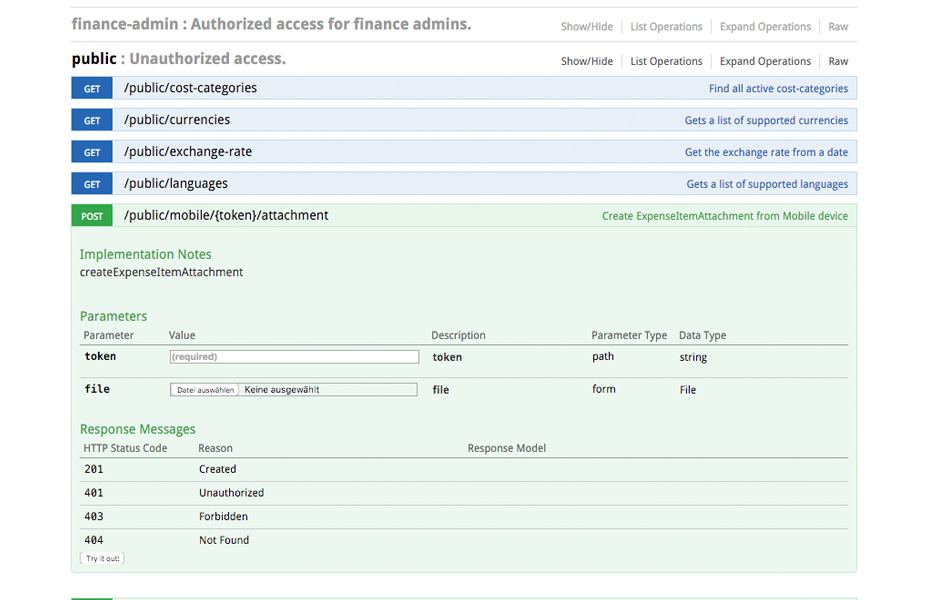
\includegraphics[width=0.80\textwidth]{swagger01}}
    \caption{Swagger: Reimbursement GUI}
    \label{fig:swagger01}
\end{figure}

\subsection{Frontend}

\subsubsection{AngularJS}
AngularJS is a client-side JavaScript framework. Its data binding and dependency injection reduces the amount of code need to be written. Further it uses templates for HTML templates and an routing to create interactive GUI's. Angular uses an MVC approach and is easy to integrate with REST services. \cite{angular}   

\subsubsection{Bootstrap}
Bootstrap is a framework consisting of HTML, CSS and JavaScript that can be used to create appealing graphical user interfaces from a design perspective. It is supported by most of the desktop and mobile web browsers available. The tool uses Bootstrap v. 3.3.5. \cite{bootstrap}

\subsubsection{Bower}
Bower is a dependency manager for JavaScript web applications like AngularJS. It keeps track of the used assets, frameworks, libraries, etc. \cite{bower}  

\subsubsection{Grunt}
Grunt is a JavaScript task runner. We use it for our frontend build. Its plugin directory supports a lot of modules to optimize the development workflow. Code-uglifying, concating, sass-compiling, file operations, autoprefixing etc. \cite{grunt} 

